\chapter{Fundamentação}
    \label{chp:Fundamentos}

	\section{Controladora Robótica Aberta}
	
        Algumas tentativas feitas pela academia foram relatadas na literatura no sentido de abrir a estrutura de controle de alguns robôs industriais~\cite{ROBERTI:2010}. Recentemente, alguns fabricantes de robôs perceberam essa demanda por parte das instituições de ensino e pesquisa e, de forma semelhante ao que vem acontecendo com os softwares de código aberto do \textit{ROS} (Sistema Operacional Robótico, em tradução livre), passaram a oferecer a opção de abertura do sistema de controle de robôs~\cite{KUBUS:2010}, isto é, uma controladora aberta. 
        
        Uma opção para atender essa demanda foi desenvolvida pelo fabricante de robôs industriais \textit{Comau}, adicionando uma arquitetura complementar à controladora de seus robôs, a \textit{Comau C5G}. Essa extensão, denominada \textit{Comau C5G Open Controller}, é feita através da conexão da controladora a um computador industrial externo, denominado \ac{LPC}, por intermédio de uma conexão \textit{Ethernet PowerLink}, como é mostrado na Figura~\ref{controladora2}~\cite{ANTONELLI:2010}.
        
        A Figura~\ref{controladora} permite a visualização da solução fornecida pelo fabricante, sendo que, a conexão \textit{Ethernet} \ac{TCPIP} precisa ser intermediada por um modem, roteador ou \textit{switch} não fornecido nessa extensão.
        
        \begin{figure}[ht]
            \centering
            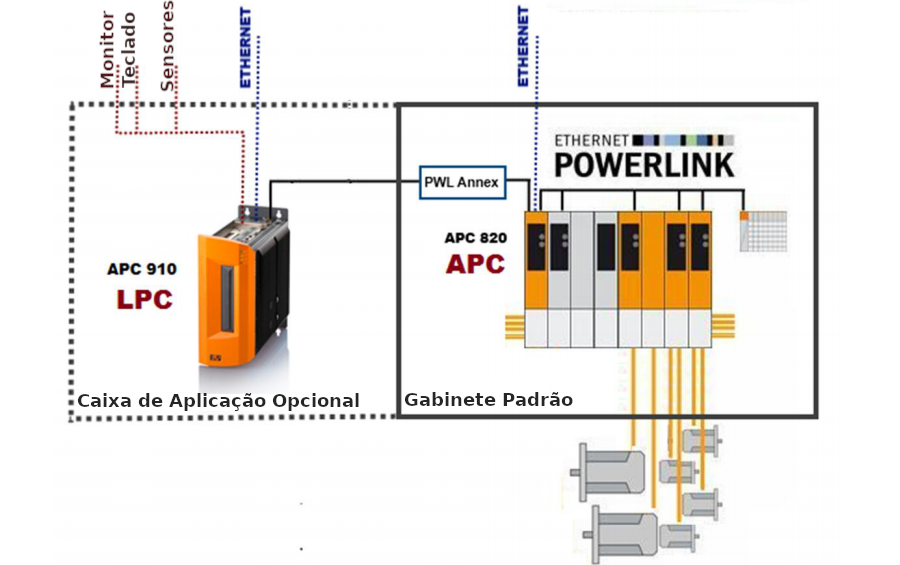
\includegraphics[width=\columnwidth]{imagens/Conexoes/controladora2.png}
            \small 
            \centering 
            \caption{Visão geral sobre o hardware do sistema C5G-Open}
            Adaptado de~\cite{Ferrara:2013}
            \label{controladora2}
        \end{figure}
        
        Assim, é possibilitado à controladora do robô industrial enviar dados sensoriais e receber referências de um software a ser programado pelo usuário, a taxas de até 1 pacote a cada \SI{0,4}{\milli\second} (1 pacote contém todas as leituras de sensores do robô). Isso possibilita a criação de softwares que implementem malhas de controle adicionais como: controle de força, visão computacional, entre outros.~\cite{Ferrara:2013}
        
        \begin{figure}[ht]
            \centering
            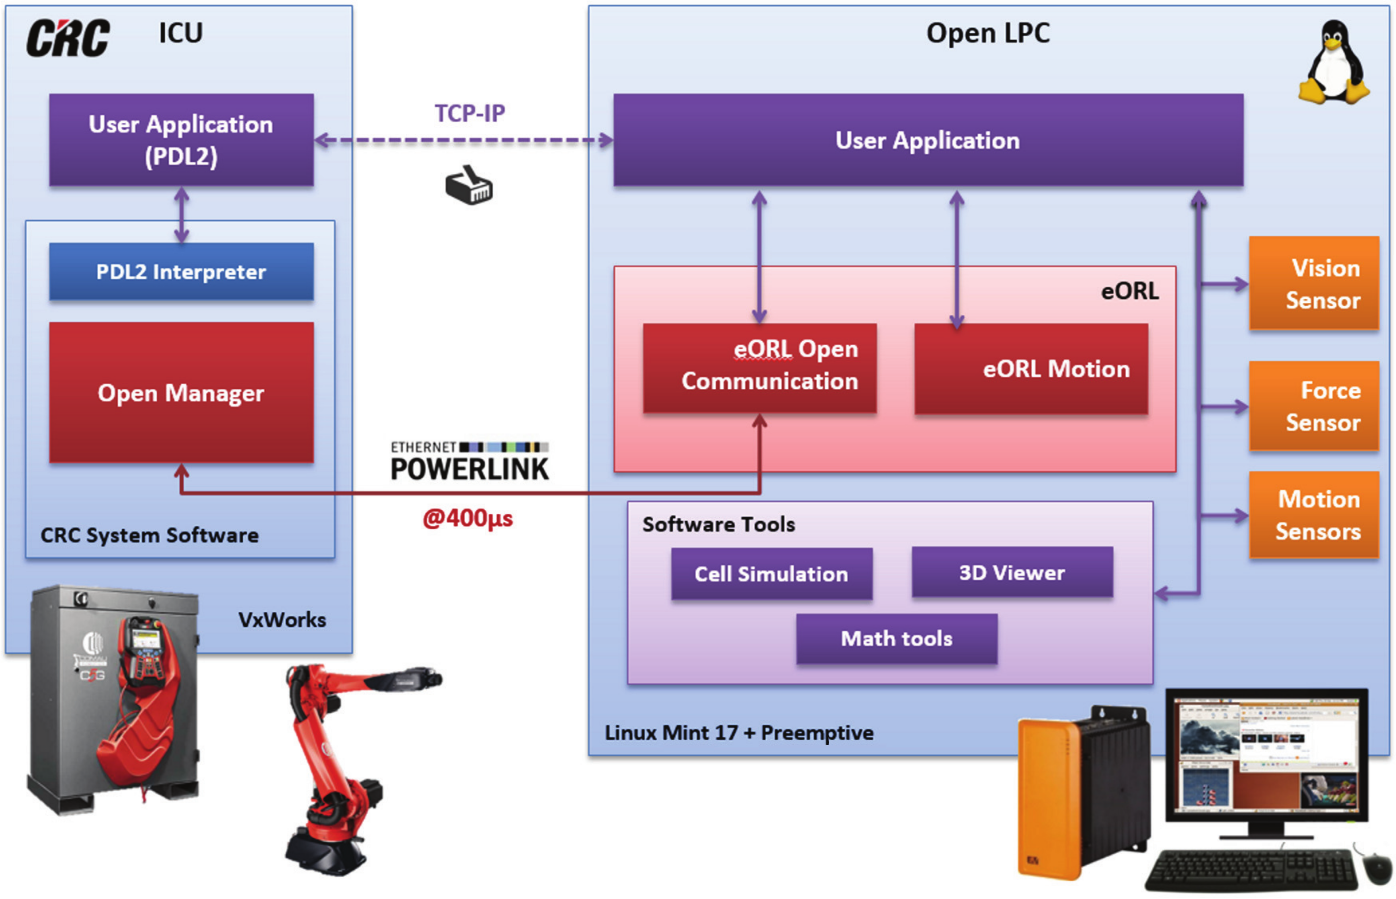
\includegraphics[width=\columnwidth]{imagens/Conexoes/controladora.png}
            \small 
            \centering 
            \caption{Visão geral do software do sistema C5G-Open}
            Fonte:~\cite{Open:Manual}
            \label{controladora}
        \end{figure} 
        
        Entretanto, existem algumas limitações, por exemplo: o software (\textit{User Application} na Figura \ref{controladora}) que implementa essa malha de controle adicional precisa ser compilado e executado nesse computador industrial externo, rodando o sistema operacional \textit{Linux Mint 17} compilado para arquitetura x86, conectado à controladora por um cabo de rede especial chamado \textit{Ethernet PowerLink} (visto na Figura \ref{controladora}). Ele precisa ser programado em C/C++ e utilizar a biblioteca proprietária de código fechado desenvolvida pela \textit{Comau} chamada \ac{eORL}, para controlar a comunicação.%Citar manual c5gopen
        
        Além disso, uma utilização inadequada por um usuário que deixe a conexão com o \ac{LPC} habilitada do lado da controladora e que não tenha a adequada resposta do lado do \ac{LPC}, por exemplo, poderá produzir um erro de comunicação que acabará sendo armazenado em seus registros e impedirá a liberação dos \textit{drivers} da controladora pelo seu módulo de gerenciamento de segurança, chamado C5G-SDM (Módulo de Distribuição e Segurança, em português)~\cite{C5G:Manual}, como já aconteceu na controladora do Laboratório de Robótica do CEFET-MG uma vez.
        
        Por fim, nem todos os programas necessários para o desenvolvimento de aplicações podem ser instalados no \ac{LPC}, como é o caso do \textit{ROS}, devido ao fato que os drivers do Powerlink Card precisam de uma versão mais antiga do Sistema Operacional Ubuntu (ou derivados dele, como Linux Mint) para funcionar~\cite{Bisson:2014}. Atualmente é executado no \ac{LPC} a versão 17 do Linux Mint, que é baseado na versão \ac{LTS} de 2014 do Ubuntu. Então, todos os programas e versões de bibliotecas do sistema operacional são versões ultrapassadas e, geralmente, não oferece suporte à instalação das novas versões dos mesmos, como é o caso do \textit{ROS 2}, que é a mais nova versão do \textit{ROS}.
        
        Para utilizar o sistema \textit{Open} é necessário a instalação da biblioteca \ac{eORL} no \ac{LPC} na mesma versão da \ac{eORL} da controladora~\cite{Open:Manual}. Além disso, é necessário habilitar o modo Open nos eixos desejados através da controladora antes de utilizar a modalidade. Para isso, é usado o programa \textit{Crcopen} disponível na controladora, conforme indicado na Figura~\ref{habilitar-open}.
        
        \begin{figure}[ht]
            \centering
            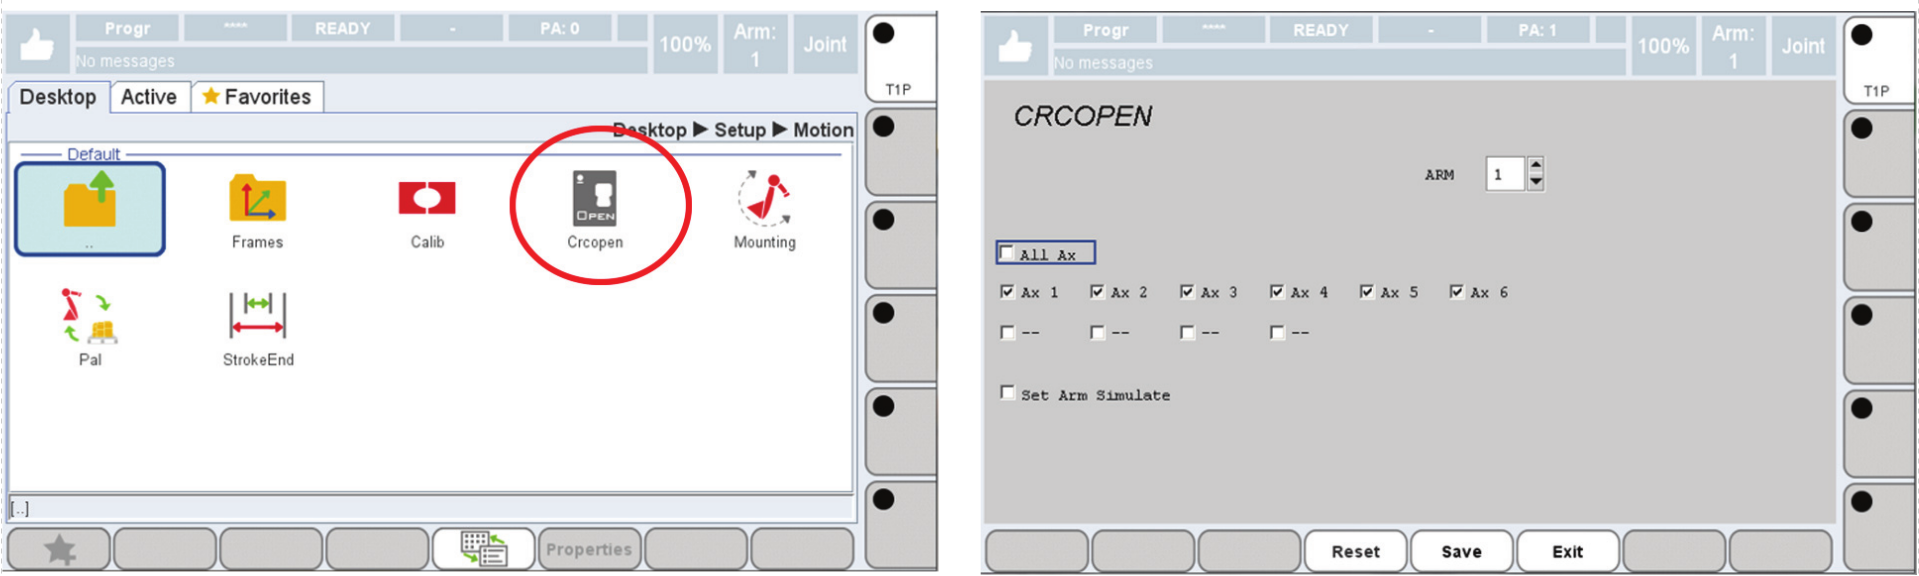
\includegraphics[width=\columnwidth]{imagens/Softwares/habilitar-open.png}
            \small 
            \centering 
            \caption{Procedimento para habilitar o modo Open dos eixos do robô~\cite{Open:Manual}}
            \label{habilitar-open}
        \end{figure}
        
    \section{Modo de Simulação}
        
        %Estou escrevendo essa subseção agora, depois você revisa
        A fabricante da controladora desenvolveu um modo de simulação para realizar testes com segurança das tarefas a serem preparadas no sistema Open. Este modo de simulação envia um comando para os controladores dos motores não atuarem nos motores e não lerem os sensores. Ao invés disso, ele irá usar a resposta esperada dos motores para estimar os valores dos respectivos sensores. Desta forma o robô permanece seguro sem se mover até que seja reiniciado o robô sem o modo de simulação.
        
        \begin{figure}[!htb] 
            \centering
            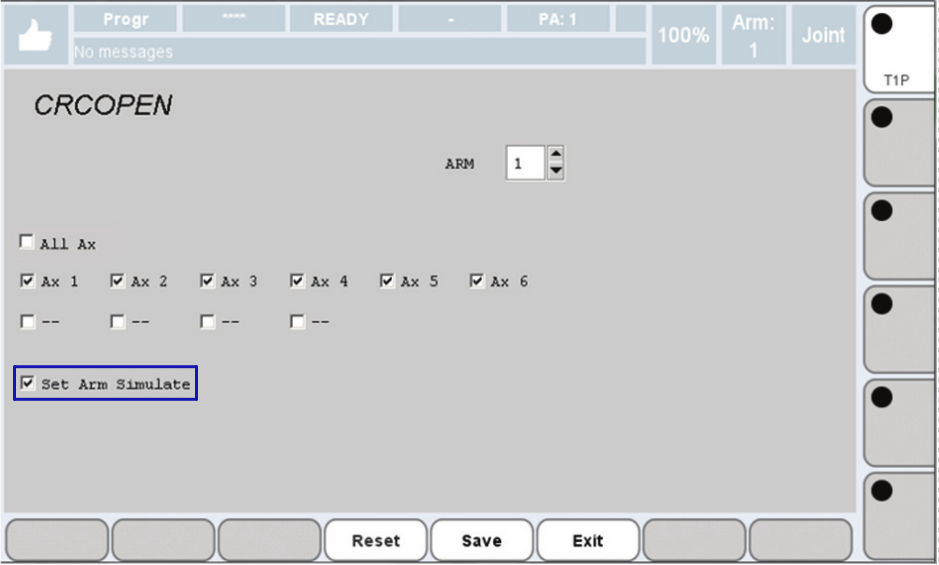
\includegraphics[width=10cm]{imagens/Softwares/habilitar-simu.png}%\columnwidth
            \small
            \centering
            \caption{Ativando o modo de simulação. Adaptado de~\cite{Open:Manual}}
            \label{fig:habilitar_simu}
        \end{figure}
        
        Existem três maneiras de visualizar os ângulos das juntas do robô no modo simulação: através da janela do programa MOTION no \ac{TP}; ou através da aplicação a ser desenvolvida pelo usuário do sistema Open (nesse caso, os pacotes de dados sensoriais que o \ac{LPC} irá receber na verdade conterão as estimações dos ângulos das juntas); ou através de um software chamado \textit{Comau Visual3D}, desenvolvido pela fabricante com a finalidade de visualizar virtualmente o robô, simulado ou não.
        
        O \textit{Visual3D} comunica-se diretamente com a controladora através da rede Ethernet, a qual a controladora está conectada, e possui o armazenado na memória dos modelos 3D de vários robôs da fabricante. Quando ele se comunica com a controladora pela primeira vez, ele recebe a informação de qual robô está conectado à controladora. Então, passa a receber continuamente os valores angulares de cada junta do robô, usando esses dados para realizar, em tempo real, uma renderização 3D do modelo do robô na \ac{POSE} determinada por esses valores. Na Figura~\ref{fig:visual} são mostrados exemplos de visualização fornecidos pelo do programa \textit{Visual3D} exibindo o robô virtual.
        
        \begin{figure}[h]
            \centering
            \begin{subfigure}[b]{0.4\textwidth}
                \centering
                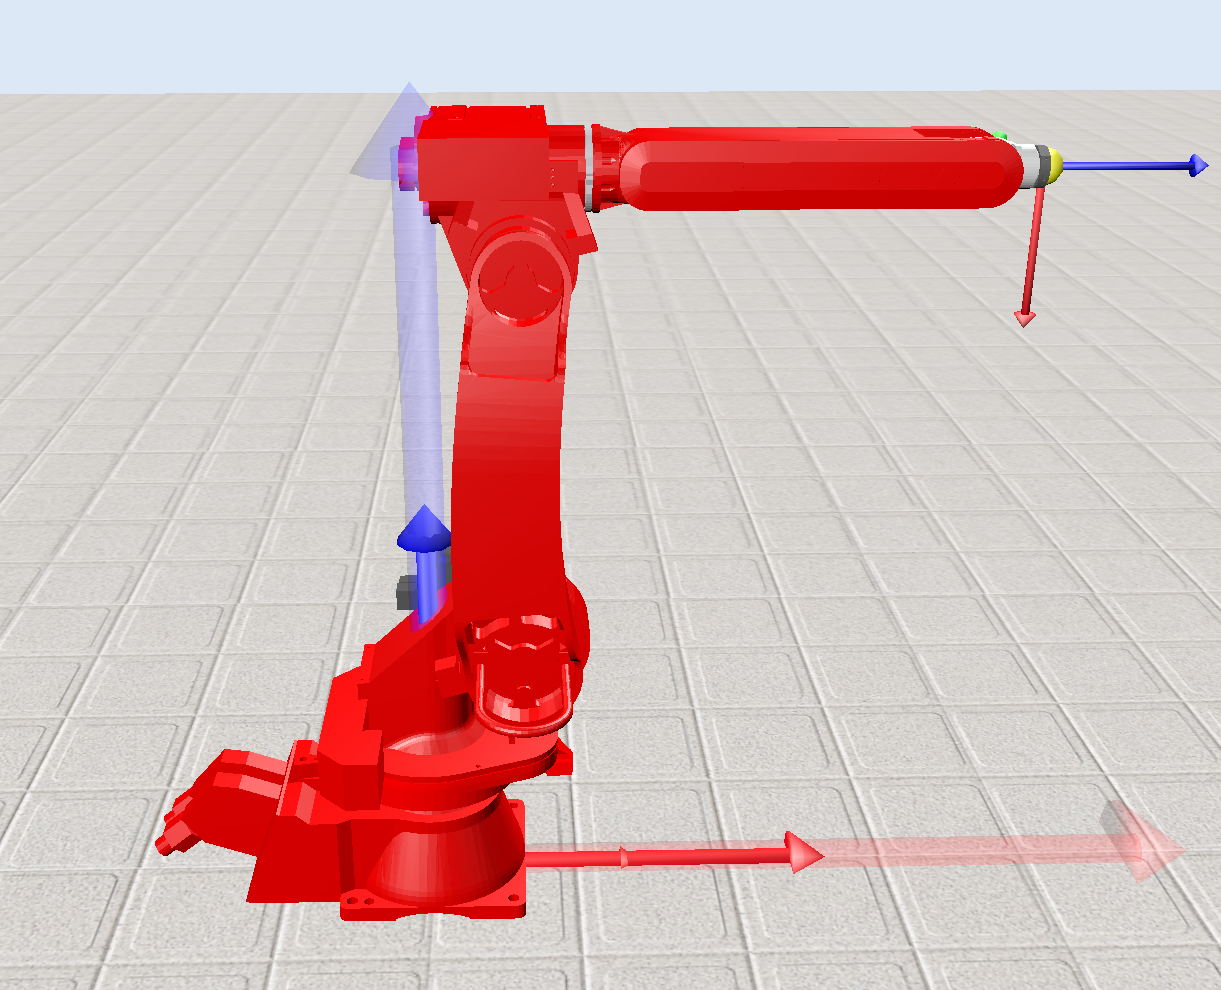
\includegraphics[width=60mm]{imagens/Softwares/visual3d-a.png}
                \caption{}
                \label{fig:visuala}
            \end{subfigure}
            \hfill
            \begin{subfigure}[b]{0.4\textwidth}
                \centering
                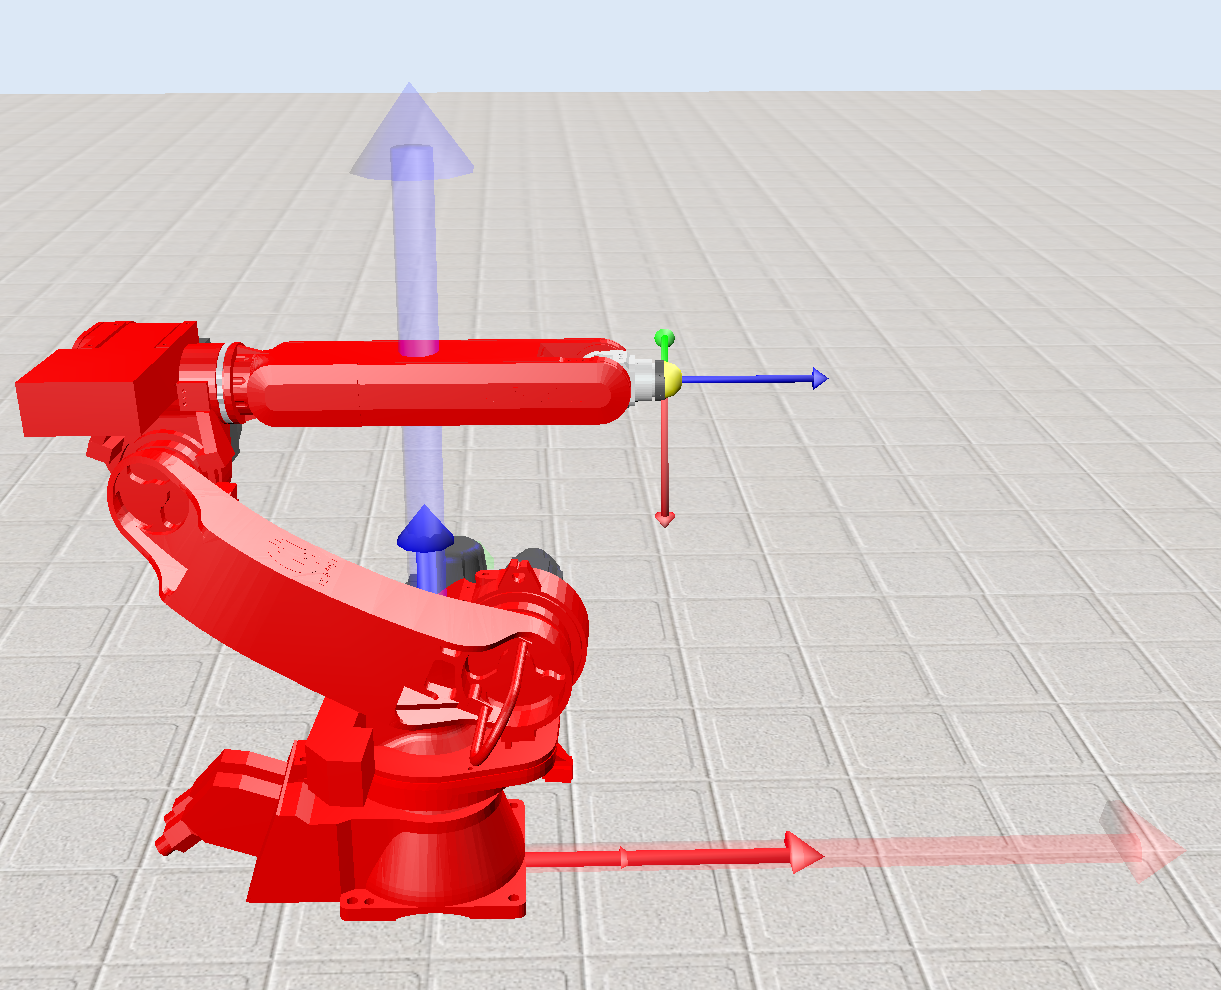
\includegraphics[width=60mm]{imagens/Softwares/visual3d-b.png}
                \caption{}
                \label{fig:visualb}
            \end{subfigure}
            \caption{Modelo 3D do robô no software Visual3D em duas \ac{POSE}'s distintas}
            \label{fig:visual}
        \end{figure}
        
        Como este programa apenas oferece uma visualização gráfica do robô para o usuário, ele não é necessário para utilizar o sistema Open ou o modo de simulação. No entanto, o \textit{Visual3D} é de grande auxílio nos testes de programas desenvolvidos para o sistema Open em modo de simulação, pois permite identificar mais facilmente se o teste simulado está ocorrendo conforme esperado, do que analisando os valores dos ângulos ou da pose do robô no \ac{TP}.
    
    \section{Ponteiro Inteligente}

        Um ponteiro inteligente é um tipo de dado implementado na linguagem de programação \textit{C++} partir da revisão \textit{C++11}. Esse tipo de dado fornece recursos adicionais aos ponteiros, como gerenciamento automático de memória. No caso, eles controlam automaticamente a memória para a qual apontam e deletam automaticamente o objeto apontado após a utilização, por exemplo, porque o proprietário é uma variável local, e a execução sai do escopo da variável.~\cite{cppreference}
        
        O Ponteiro Inteligente utilizando no desenvolvimento deste trabalho é o shared\_ptr. Ele é um ponteiro compartilhado e tem a característica de nenhum shared\_ptr específico possuir algum objeto. Todos os shared\_ptr que apontam para o mesmo objeto colaboram para garantir sua existência e quando todos deixam de apontar para tal objeto ele é destruído automaticamente.~\cite{meyers2015} 
        